\subchapter{First Yocto build}{Your first dive into a Yocto project and its
	build mechanism}

During this lab, you will:
\begin{itemize}
  \item Setup a Yocto environment
  \item Configure the project and choose a target
  \item Build your first Yocto image
\end{itemize}

\section{Setup}

Before starting this lab, make sure your home directory is not encrypted. Yocto
cannot be used on top of an eCryptFS file system due to limitations on file name
lengths.

Go to the \code{\$HOME/yocto-labs/} directory.

Install the required packages:
\begin{verbatim}
sudo apt-get install chrpath gawk texinfo
\end{verbatim}

\section{Set up the Ethernet communication}

Later on, we will transfer files from the development workstation to
the board using the TFTP protocol, which works on top of an Ethernet
connection.

To start with, install the \code{tftpd-hdpa} server and create the root TFTP
directory:
\begin{verbatim}
sudo apt-get install tftp-hdpa
sudo mkdir -m 777 /tftp
\end{verbatim}

Then make sure the \code{tftp-hdpa} server uses the right directory by checking
the \code{TFTP_DIRECTORY} variable in \code{/etc/default/tftpd-hpa}.

Finally restart the service to make sure all modifications are effective:
\begin{verbatim}
sudo service tftpd-hdpa restart
\end{verbatim}

With a network cable, connect the Ethernet port of your board to the 
one of your computer. If your computer already has a wired connection
to the network, your instructor will provide you with a USB Ethernet
adapter. A new network interface, probably \code{eth1} or \code{eth2},
should appear on your Linux system.

To configure this network interface on the workstation side, click on
the {\em Network Manager} tasklet on your desktop, and select {\em
  Edit Connections}.

\begin{center}
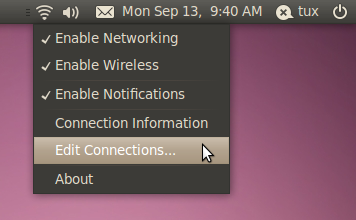
\includegraphics[width=8cm]{../labs/common/network-config-1.png}
\end{center}

Select the new {\em wired network connection}:

\begin{center}
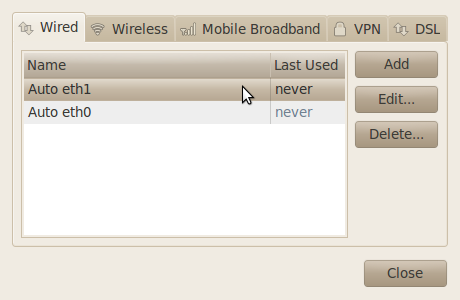
\includegraphics[width=8cm]{../labs/common/network-config-2.png}
\end{center}

In the \code{IPv4 Settings} tab, press the \code{Add} button
and make the interface use a static IP
address, like \code{192.168.0.1} (of course, make sure that this
address belongs to a separate network segment from the one of the main
company network).

\begin{center}
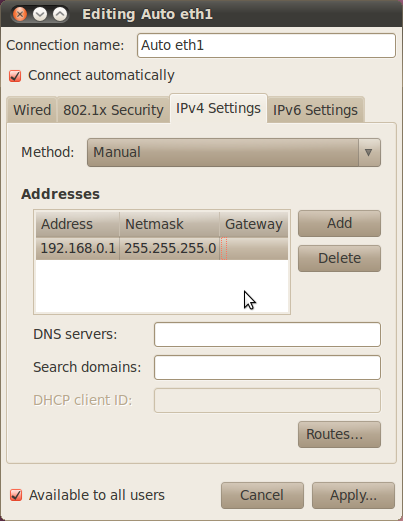
\includegraphics[width=8cm]{../labs/common/network-config-3.png}
\end{center}

You can use \code{255.255.255.0} as \code{Netmask}, and leave the
\code{Gateway} field untouched (if you click on the \code{Gateway} box, you
will have to type a valid IP address, otherwise you won't be apply to
click on the \code{Apply} button).

Now, configure the network on the board in U-Boot by setting the \code{ipaddr}
and \code{serverip} environment variables:

\begin{verbatim}
setenv ipaddr 192.168.0.100
setenv serverip 192.168.0.1
\end{verbatim}

The first time you use your board, you also need to send the MAC address
in U-boot:

\begin{verbatim}
setenv ethaddr 01:02:03:04:05:06
\end{verbatim}

In case the board was previously configured in a different way, we
also turn off automatic booting after commands that can be used to
copy a kernel to RAM:

\begin{verbatim}
setenv autostart no
\end{verbatim}

To make these settings permanent, save the environment:

\begin{verbatim}
saveenv
\end{verbatim}

Now switch your board off and on again\footnote{Power cycling your
  board is needed to make your \code{ethaddr} permanent, for obscure
  reasons. If you don't, U-boot will complain that \code{ethaddr} is not
  set.}.

You can then test the TFTP connection. First, put a small text file in
the directory exported through TFTP on your development
workstation. Then, from U-Boot, do:

\begin{verbatim}
tftp 0x80000000 textfile.txt
\end{verbatim}

{\bf Caution: known issue in Ubuntu 12.04 and later}:
if this command doesn't work, you may have to stop the server
and start it again every time you boot your workstation:

\begin{verbatim}
sudo service tftpd-hpa restart
\end{verbatim}

The \code{tftp} command should have downloaded
the \code{textfile.txt} file from your development
workstation into the board's memory at location 0x80000000 (this
location is part of the board DRAM). You can verify that the download
was successful by dumping the contents of the memory:

\begin{verbatim}
md 0x80000000
\end{verbatim}


\section{Download Yocto}

Download the latest stable version of the Yocto project and extract it:
\begin{verbatim}
wget http://downloads.yoctoproject.org/releases/yocto/yocto-1.5.1/\
  poky-dora-10.0.1.tar.bz2
tar xf poky-dora-10.0.1.tar.bz2
\end{verbatim}

Go to the Yocto root directory: \code{cd poky-dora-10.0.1}

Then download the Yocto TI layer:
\begin{verbatim}
git clone git://git.yoctoproject.org/meta-ti.git
\end{verbatim}

\section{Setup the build environment}

Export all needed variables and setup the build directory:
\begin{verbatim}
source oe-init-build-env
\end{verbatim}

In order to choose the target and to configure the generic build settings,
edit the local configuration file (\code{\$BUILDDIR/conf/local.conf}). Set
the target machine to \code{beaglebone} and update the parallelization variables
(\code{BB_NUMBER_THREADS} and \code{PARALLEL_MAKE}) according to your computer
capabilities.

Also, if you need to save disk space on your computer you can add \code{INHERIT
+= "rm_work"} in the previous configuration file. This will remove the
package work directory once a package is built.

Finally, don't forget to let the configuration aware of the TI layer. Edit the
layer configuration file (\code{\$BUILDDIR/conf/bblayers.conf}) and append the
full path to the \code{meta-ti} directory to the \code{BBLAYERS} variable.

\section{Build your first image}

Now that you're ready to start the compilation, simply run:
\begin{verbatim}
bitbake core-image-minimal
\end{verbatim}

Once the build finished, all output images can be find under
\code{\$BUILDDIR/tmp/deploy/images/beaglebone}.

\section{Setup the internal eMMC}

In order to boot from the internal eMMC, we should make sure it is properly
setted up before writing our images.

\section{Flash the board}

In order to boot the BeagleBone Black we will flash the bootloader and the
kernel image in the internal eMMC here.

On the training computer copy the bootloader, kernel and rootfs images in the
root TFTP directory:
\begin{verbatim}
cp $BUILDDIR/tmp/deploy/images/beaglebone/{MLO,u-boot.img,zImage} /tftp
\end{verbatim}

Then retrieve these files on the BeagleBone Board memory. We will first download
the first stage bootloader, the \code{MLO}:
\begin{verbatim}
tftp 0x80200000 MLO
\end{verbatim}

Finally flash this file into the internal eMMC:
\begin{verbatim}
TBD
\end{verbatim}
